\chapter{Data Foundation}
\label{data}
In this chapter the provided datasets from the previously mentioned street information systems and the FCD provider will be elaborated. First an overview of FCD in general and the available dataset is given. To give an overview about what results can be expected the incident datasets from BAYSIS and ArbIS are presented with descriptive statistic. The most relevant parameters of the datasets will be elaborated and illustrated. The parameters are also categorized in the variable types, defined in chapter \autoref{correlation_variable_types}.

\section{FCD}
\label{dataset_fcd}
 
As described in chapter 1.1, \acrshort{fcd} represents the movement of vehicles and can be used to calculate vehicle speeds and trajectories. The provided dataset contains the aggregated absolute and relative speeds for the highways and state streets, calculated from \acrshort{fcd} data. The process of speeds estimation with \acrshort{fcd} data is explained in detail by Felix Rampe in chapter 4 of his thesis \textit{Traffic Speed Estimation and Prediction Using Floating Car Data} \parencite{Rempe2018}, but is outside of the scope for this thesis. The FCD is mapped onto the HERE \parencite{HERE2020} network, to be compliant with the geolocation system used in the project.

% TODO add more info about FCD if there is time 
% https://athene-forschung.unibw.de/doc/127445/127445.pdf
% Traffic Speed Estimation and Prediction Using Floating Car Data.pdf

Each of these aggregated speeds now represents the mean speed over a three minute time interval on the corresponding road section. This arrangement of speeds for each time step and space step is called speed matrix and is the base data for the congestion detection. Figure \autoref{img:speedMatrixPlot_mutipleMixedClusters} shows a visual representation a speed matrixes with the horizontal axes being the spatial extend and the vertical axes the time extend. Deep greens represent free flowing traffic with ~130 km/h, which is the norm speed in Germany (in German called “Richtgeschwindigkeit”) on highways set the legislator. The speed scale then develops linearly downwards deep red indicating traffic with 30 km/h or less. 

\begin{figure}[ht]
	\centering
	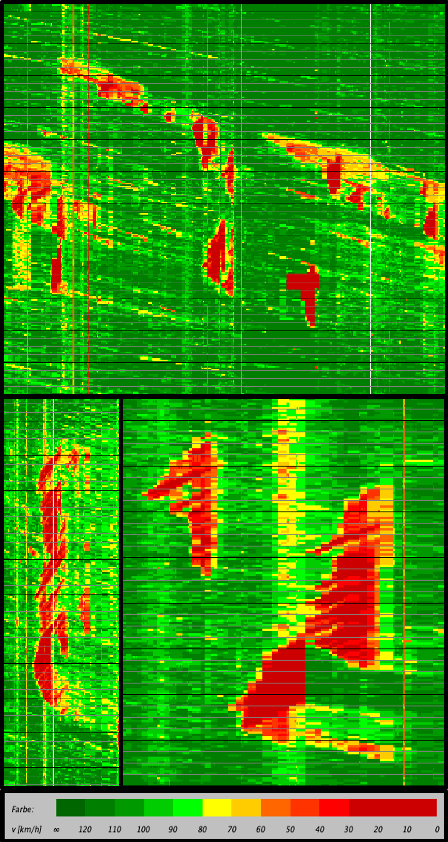
\includegraphics[scale=0.7]{images/SpeedMatrixPlot_mutiple}
	\caption{Speed matrix plots of processed FCD data, showing different jam clusters}
	\label{img:speedMatrixPlot_mutipleMixedClusters}
\end{figure}

The observer will clearly recognize the jams represented by the clusters of red and orange cells in the figure \autoref{img:speedMatrixPlot_mutipleMixedClusters}, with the angled extends towards the right down edge, due to the vehicle trajectory through space and time. These cluster, also shown in the two lower pictures, which representing one or multiple jams can be densely packed or spotted into smaller clusters or, depending on the severity of a jam can be seen, by the cluster which contain more orange or yellow cells than red. 

From this visual clarity, the continuity of the data points and the precision on 3-minute intervals it can concluded that a comprehensive algorithmic approach should be able to detect such congestion events. This being said, the dataset does contain defects in the form of missing values for complete road sections, which can interfere with detection algorithm. Another defect type are obviously wrong speed block, meaning sudden speed drops or jumps to areas of identical speeds with an abnormal temporal and spatial extend, which have to be ignored during processing. 

\section{BAYSIS}
\label{dataset_baysis}

The \acrfull{baysis} as describe in chapter \autoref{dataset_baysis}, collects a wide range of different information types, one of then being accidents with the corresponding police reports. Accidents have a strong traffic influence on the Bavarian street network, with more than 400.000 being recorded in the year 2019 (StMi, 2020), hence their importance in this topic. The provided export from BAYSIS contains all accidents of the year 2019 on the Bavarian highway network, which are 10262 records in number. 

Each accident report includes a variety of specifications, which covers environmental indicators like weather or light situation, accident characteristics like accident type, collision object or cause, as well as information over the involved like nationality, age and gender. In total, one report contains 132 values, describing the accident, participant and environment. Because we do not want to form a stereotype of accident participant but rather find significant accident characteristics or environmental factors most of the descriptive values for the involved persons are not considered. Variables without any values or single values are also neglected. To meet a statistical significant result a diverse distribution in the values would be preferred, to reduce the risk of uncertain relation. Because the correlation of a non distributed variable, which for example has one values occupying a 95\% major share, is based on a sample set comprised of mostly the same samples, the interpretability for a correlation to other values but the major share is very limited (see \autoref{correlation_significance_uncertainty} for more detailed elaboration of this assumption).

From this curtailed pool of correlate able and analyze able characteristics all parameters that have a logical significance with causes or effects of an accident will be considered in the analysis.  The referred diagrams are available as larger prints in the appendix \autoref{appendix_baysis} for better readability. 

\begin{figure}[ht]
	\centering
	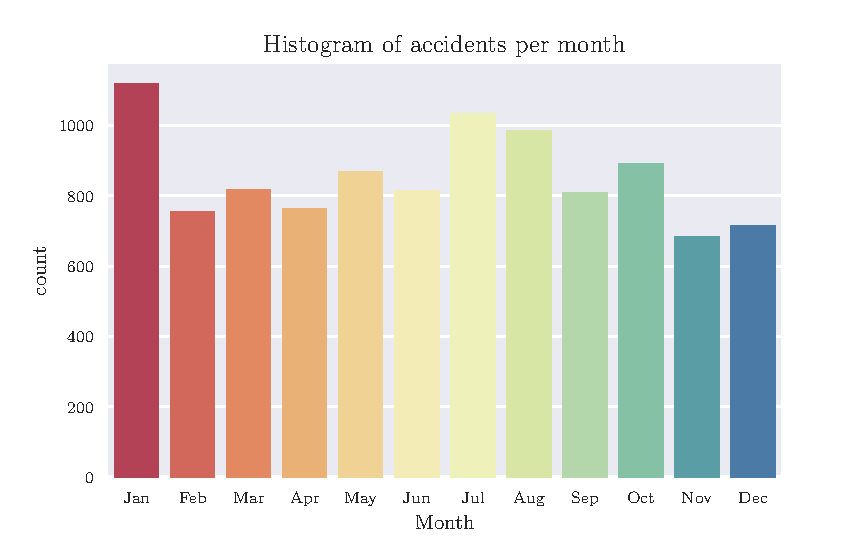
\includegraphics[scale=0.9]{CorrAnalysis/data/BAYSIS/01_dataset/plots/baysis_dataset_hist_month}
	\caption{Monthly distribution of accident counts}
	\label{img:baysis_dataset_dist_month}
\end{figure}

A look on the monthly distribution of accidents recorded by BAYSIS (see figure \autoref{img:baysis_dataset_dist_month}) shows that that the months of January, July and August have considerably higher number of accidents, with respectively 31\,\%, 21\,\% and 15\,\% increase over the mean count of 855 accidents per month. The increased number in January can be explained with the increased number of accidents due to ice and snow conditions, which reduces traction on roads and can lead to uncontrollable vehicle behavior. Also the reduced visibility during snow falls increases accident numbers. In July and August the increased traffic volume because of public holidays is the most probable explanation for the higher number of accidents. Another valuable distribution is the number of accidents per road (see figure \autoref{img:baysis_dataset_dist_highway}). The roads A3, A9 and A8 have relative high count of accidents. In contrast the road A71 and downwards have only an accidents and therefore have a high uncertainty associated with them. 

\begin{figure}[ht]
	\centering
	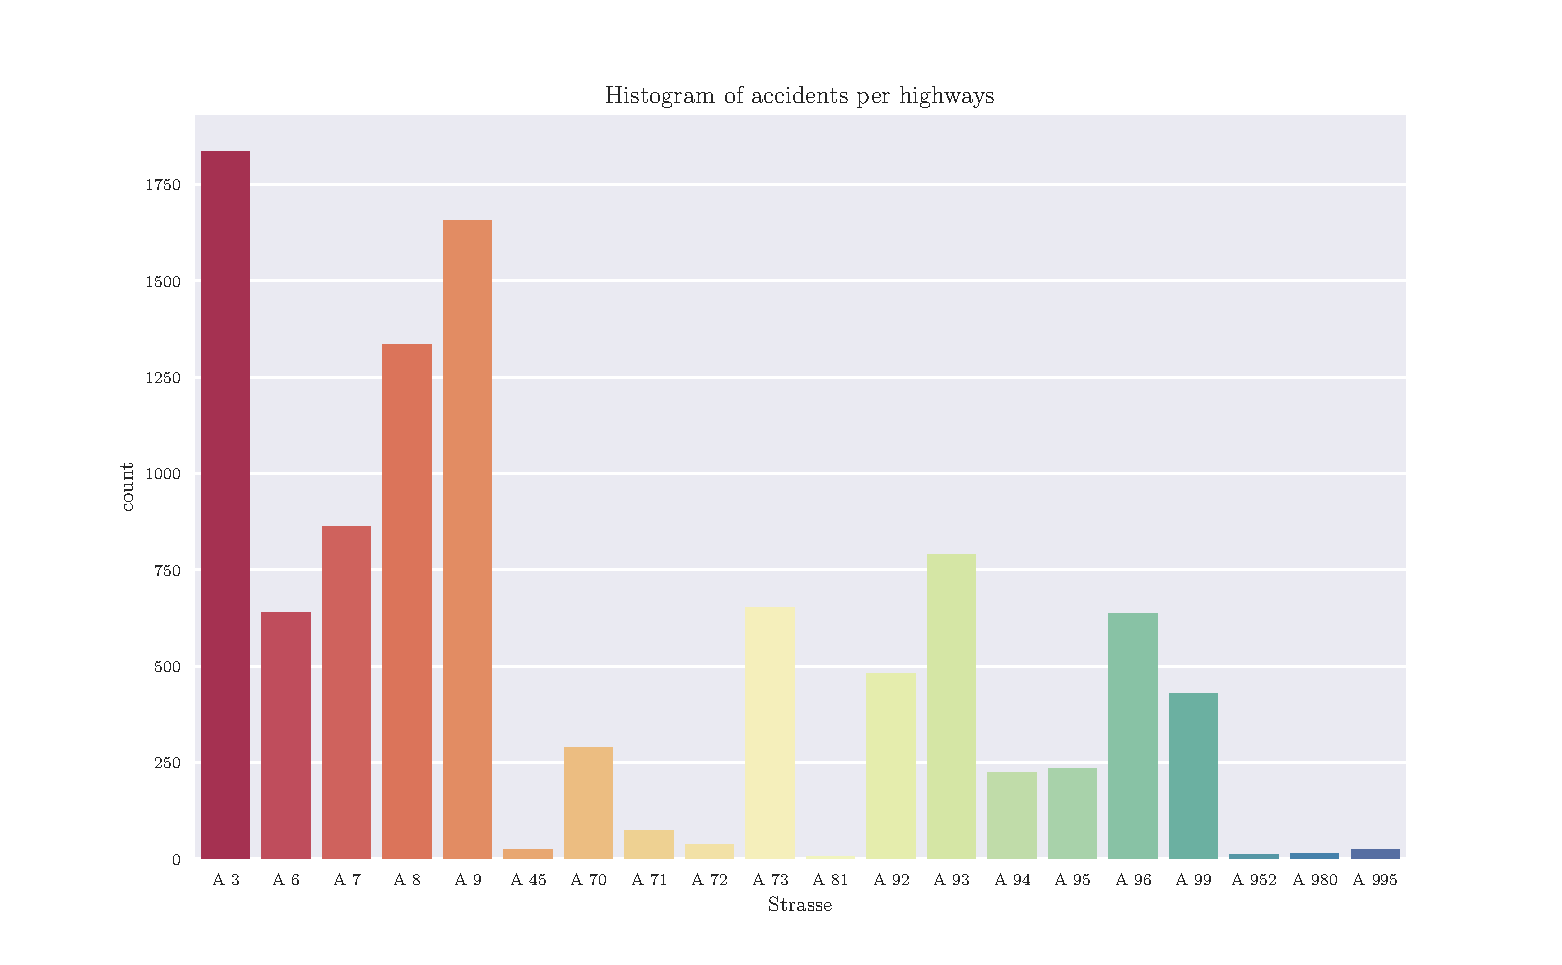
\includegraphics[scale=0.8]{CorrAnalysis/data/BAYSIS/01_dataset/plots/baysis_dataset_hist_highway}
	\caption{Distribution of accident counts, by road}
	\label{img:baysis_dataset_dist_highway}
\end{figure}

\paragraph{Kat}
The accident category (shown in figure \autoref{img:baysis_dataset_kat_typ_betei} and table \autoref{table:baysis_dataset_Kat}), describes the which damages or injuries can be associated with the accident. It ranges from accident with just  damaged property, lightly and heavily injured to deathly accidents. The distribution develops from lowest to highs counts, in order of gravity of the category. The variable consists of four values, which can be ordered, and is therefore ordinal.
\noindent
\begin{table}[ht]
	\centering
	\begin{tabular}{c|l}  
 		0 & Minor Accident  \\
 		1 & Accident with deaths  \\ 
 		2 & Accident with heavily injured  \\
 		3 & Accident with lightly injured  \\
 		7 & Accident with property damage  \\
	\end{tabular}
	\caption{Identifier and description of 'Kat'}
	\label{table:baysis_dataset_Kat}
\end{table}

\paragraph{Typ}
The accident type variable (shown in figure \autoref{img:baysis_dataset_kat_typ_betei} and table \autoref{table:baysis_dataset_Typ}) incorporates different kind of traffic movements, from straight driving to turning movements or merging. It describes during which kind of movement the accident happened. Beside of an 80\,\% share of accidents related to driving or straight driving situations, the parameter does not indicate any other features. The variable does not show any order and is therefore of nominal type.
\noindent
\begin{table}[ht]
	\centering
	\begin{tabular}{c|l}  
 		1 & Driving accident  \\ 
 		2 & Turning accident  \\
 		3 & Merging / Crossing accident  \\
 		4 & Crossing over accident  \\
 		5 & Accident in standing traffic  \\
 		6 & Accident in straight traffic  \\
 		7 & Other  \\
	\end{tabular}
	\caption{Identifier and description of 'Typ'}
	\label{table:baysis_dataset_Typ}
\end{table}

\paragraph{Betei}
The distribution of the number of involved persons (shown in figure \autoref{img:baysis_dataset_kat_typ_betei}) shows that more than 96\,\% of accidents have three or less involved persons. The major share of two involved persons makes up for 56\,\% and the second biggest of one involved person for 30\,\% of the total count. Because of the increasing order of values, the variable is of ordinal type.

\pagestyle{empty}
\begin{figure}[!ht]
	\centering
	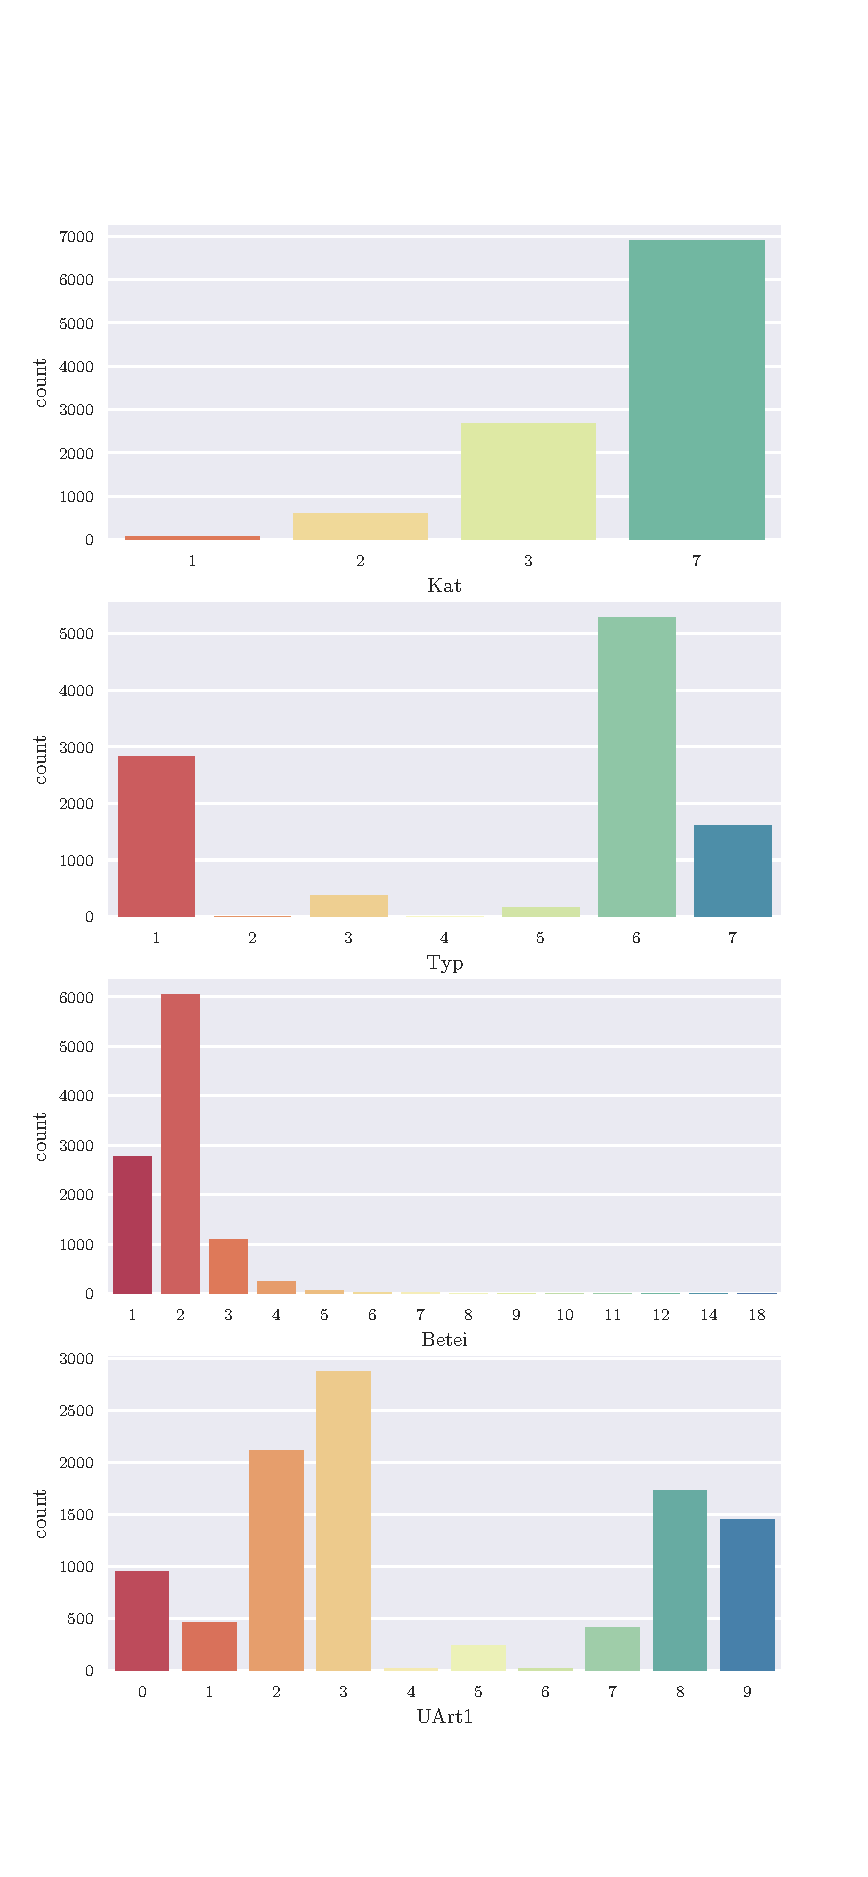
\includegraphics[scale=0.7, trim=0cm 1.5cm 0cm 1cm]{CorrAnalysis/data/BAYSIS/01_dataset/plots/baysis_dataset_count_multiple01}
	\caption{Distribution of the accident category Kat, Typ and Betei}
	\label{img:baysis_dataset_kat_typ_betei}
\end{figure}
\pagestyle{headings}

\paragraph{UArt}
The accident cause type, described by the two aggregated variables UArt1 and UArt2 (shown in figure \autoref{img:baysis_dataset_UArt_AUrs_AufHi} and table \autoref{table:baysis_dataset_UArt}), presents two major sets of causes. One being the accidents with waiting, stopping and starting vehicles in the same lane, which describe typical collision accidents during congested traffic. The other being the accidents in the next left or right lane, which describe common lane changing collisions. Accidents with cross traffic, pedestrians or opposite traffic are relatively uncommon. The variable does not show any order and is therefore of nominal type.
\noindent
\begin{table}[ht]
	\centering
	\begin{tabular}{c|l}  
 		1 & Collision with starting, standing or stopping vehicle  \\ 
 		2 & Collision with ahead and waiting vehicle  \\
 		3 & Collision with vehicle on separate lane in same direction  \\
 		4 & Collision with vehicle going in opposite direction  \\
 		5 & Collision with turning or crossing vehicle  \\
 		6 & Collision between vehicle and pedestrian  \\
 		7 & Collision with obstacle  \\
 		8 & Deviation to the right  \\
 		9 & Deviation to the left  \\
 		0 & Other  \\
	\end{tabular}
	\caption{Identifier and description of 'UArt'}
	\label{table:baysis_dataset_UArt}
\end{table}

\paragraph{AUrs}
The summarized distribution of the parameters “AUrs1” and “AUrs2” (shown in figure \autoref{img:baysis_dataset_UArt_AUrs_AufHi} and table \autoref{table:baysis_dataset_AUrs}) shows that only the first category of “Slippery road condition due to oil” hold a significant share. Because of that any correlation to this parameter needs to interpreted with caution, die the the high uncertainty. The variable is of nominal type.
\noindent
\begin{table}[ht]
	\centering
	\begin{tabular}{c|l}  
	70 & Slippery street due to oil \\
	71 & Slippery street due to dirt \\
	72 & Slippery street due to snow or ice \\
	73 & Slippery street due to rain \\
	74 & Slippery street due to other objects \\
	75 & Cart rut due to rain, snow or ice \\
	76 & Other condition of road \\
	77 & Un regular condition of traffic signs \\
	78 & Bad lighting of street \\
	79 & Bad safety on train crossing \\
	80 & Visibility issues due to fog \\
	81 & Visibility issues due to rain or hail \\
	82 & Visibility issues due to sun or glare \\
	83 & Crosswind \\
	84 & Visibility issues due to storm \\
	85 & Unsafe roadwork \\
	86 & Wild animals \\
	87 & Other animals \\
	88 & Other obstacles \\
	89 & Other causes \\
	\end{tabular}
	\caption{Identifier and description of 'AUrs'}
	\label{table:baysis_dataset_AUrs}
\end{table}

\paragraph{AufHi}
The obstacle collision distribution (shown in figure \autoref{img:baysis_dataset_UArt_AUrs_AufHi}) reveals that in most collision accidents car hit the guardrails. The other categories are rather uncommon. With 1,5\,\% of accidents without any collision, it can be stated that in most cases a collision is part of an accident. The counts of the remaining categories are insignificant. The variable does not show any order and is therefore of nominal type.
\noindent
\begin{table}[ht]
	\centering
	\begin{tabular}{c|l}  
		0 & Single tree \\
		1 & Pillar \\
		2 & Abutment \\
		3 & Guardrail \\
		4 & Other object \\
		5 & No collision \\
		7 & Tree line or alley \\
		8 & Tree group or forest \\
		9 & Busches \\
	\end{tabular}
	\caption{Identifier and description of 'AufHi'}
	\label{table:baysis_dataset_AufHi}
\end{table}

\pagestyle{empty}
\begin{figure}[!ht]
	\centering
	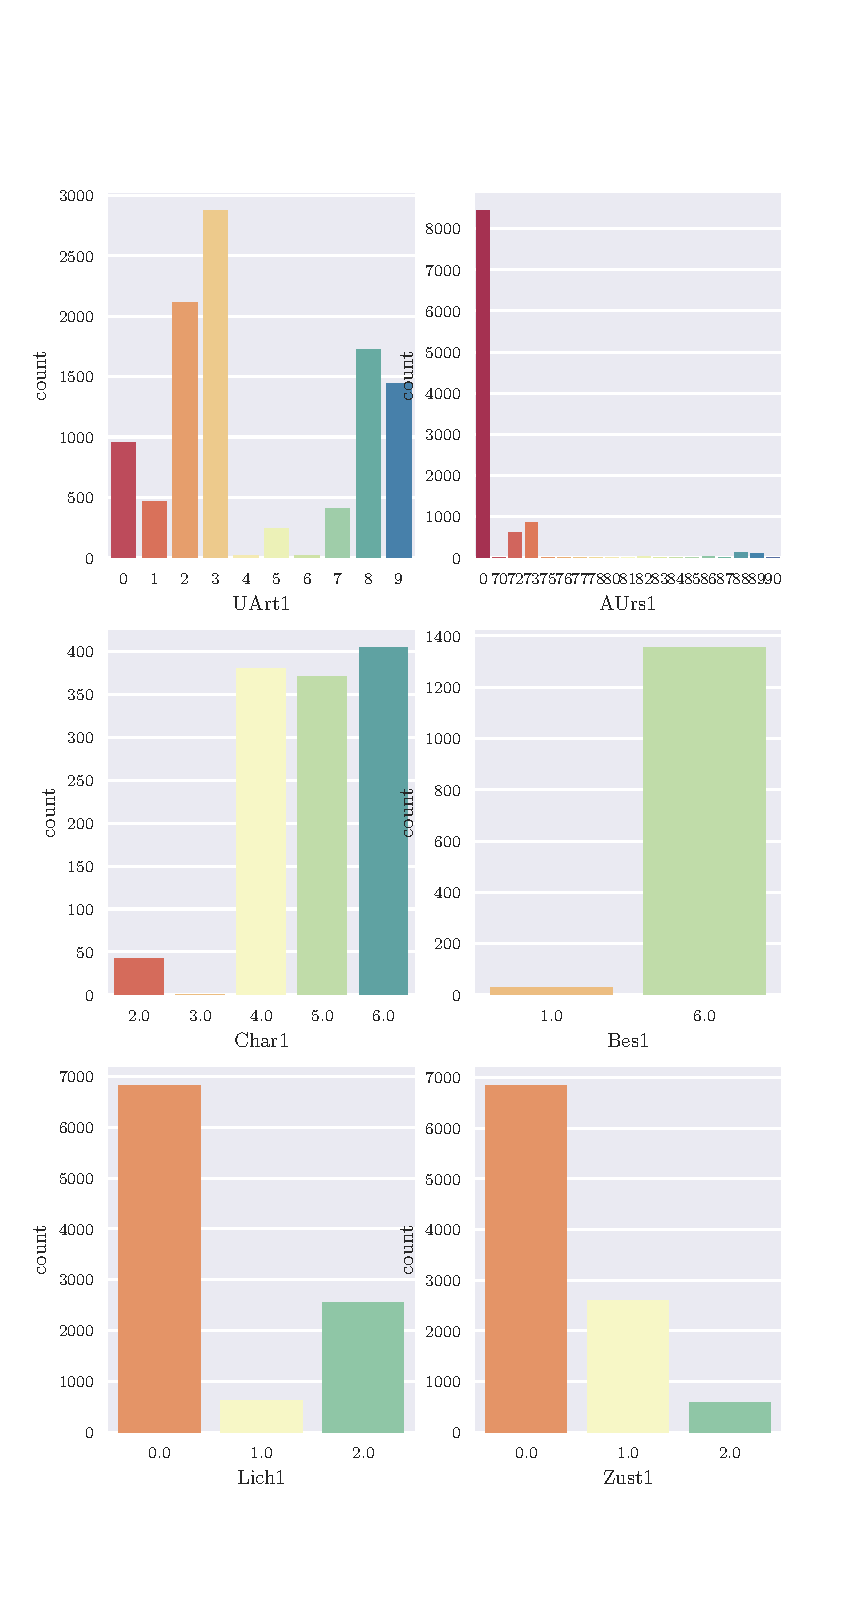
\includegraphics[scale=0.7, trim=0cm 1.5cm 0cm 1cm]{CorrAnalysis/data/BAYSIS/01_dataset/plots/baysis_dataset_count_multiple02}
	\caption{Distribution of the accident category UArt, AUrs and AufHi}
	\label{img:baysis_dataset_UArt_AUrs_AufHi}
\end{figure}
\pagestyle{headings}

\paragraph{Alkoh}
The Alcohol involvement indication parameter only contains one variables of $1$ ($yes$), whereas an empty variable referred to $no$ or $unknown$. It reveals that only 1,9\% of accidents have one or more involved persons with measurable blood alcohol. The variable only has two unique values and is therefore dichotomous.

\paragraph{Char}
The variable distribution shown in figure \autoref{img:baysis_dataset_Char_Bes_Lich} describes the characteristic of the street where the accident happened. Since we are only considering highway, the type of "Crossing", "Property" and "Roundabout" is expected to be zero. The variable is not ordered and therefore of nominal type.  
\noindent
\begin{table}[ht]
	\centering
	\begin{tabular}{c|l}  
		1 & Crossing \\
	    2 & Entry / Exit \\
	    3 & Property access \\
	    4 & Incline \\
	    5 & Decline \\
	    6 & Curve \\
	    7 & Roundabout \\
	\end{tabular}
	\caption{Identifier and description of 'Char'}
	\label{table:baysis_dataset_Char}
\end{table}

\paragraph{Bes}
The aggregated distribution of the variables "Bes1", "Bes2" and "Bes3" (shown in \autoref{img:baysis_dataset_Char_Bes_Lich}), which further defines the street characteristic mentioned above only has one significant share of the type "Roadwork". The variable itself is therefore not suitable for a correlation analysis, but can be used as validation criterium for the matching of roadwork incidents.
\noindent
\begin{table}[ht]
	\centering
	\begin{tabular}{c|l}  
		1 & Confusing \\ 
		2 & Level crossing \\
		3 & Pedestrian crossing \\
		4 & Pedestrian passage \\
		5 & Bus-stop \\
		6 & Roadwork \\
		7 & Calm traffic area \\
		8 & RAV on street \\
		9 & RAV separate \\
		0 & RAV obligatory \\
	\end{tabular}
	\caption{Identifier and description of 'Bes'}
	\label{table:baysis_dataset_Bes}
\end{table}

\paragraph{Lich}
The light situation parameter (shown in \autoref{img:baysis_dataset_Char_Bes_Lich}) does not reveal any features and describes the lighting condition when the accident happened. Because it can be ranked from best to worst lighting is is of ordinal type.
\noindent
\begin{table}[ht]
	\centering
	\begin{tabular}{c|l}  
	0 & Daylight \\
    1 & Noon \\
    2 & Darkness \\
    3 & Street lighting working \\
    4 & Street lighting not working \\
	\end{tabular}
	\caption{Identifier and description of 'Zust'}
	\label{table:baysis_dataset_Zust}
\end{table} 

\pagestyle{empty}
\begin{figure}[!ht]
	\centering
	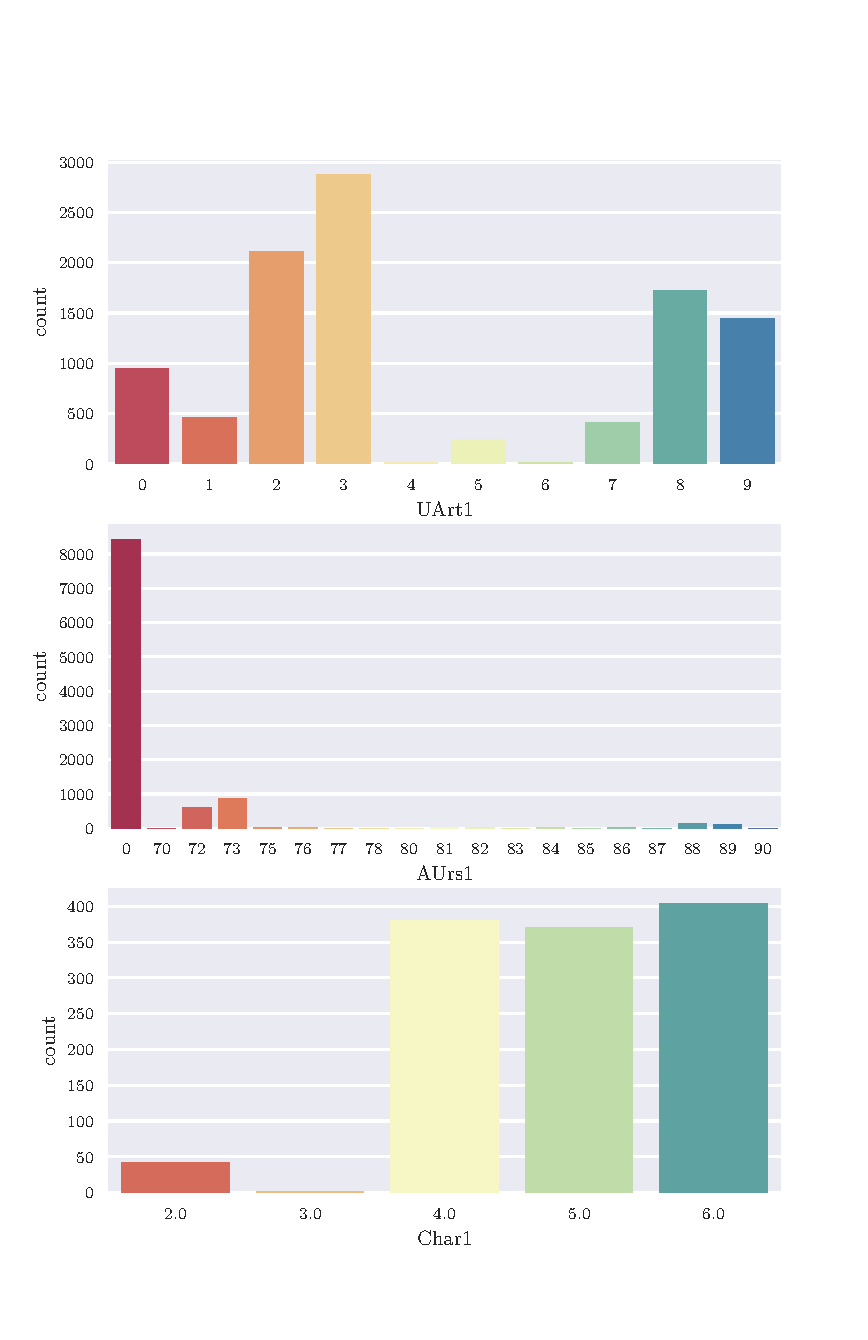
\includegraphics[scale=0.7, trim=0cm 1.5cm 0cm 1cm]{CorrAnalysis/data/BAYSIS/01_dataset/plots/baysis_dataset_count_multiple03}
	\caption{Distribution of the accident category Char, Bes and Lich}
	\label{img:baysis_dataset_Char_Bes_Lich}
\end{figure}
\pagestyle{headings}

\paragraph{Zust}
The road condition parameter (shown in \autoref{img:baysis_dataset_Zust_Fstf_WoTag}) describes in which condition the road was at time of the accident in the for of wet, dry, iced or slippery.
\noindent
\begin{table}[ht]
	\centering
	\begin{tabular}{c|l}  
		0 & Dry \\ 
 		1 & Wet \\ 
 		2 & Ice \\
 		3 & Slippery (oil, dirt, ...)  \\
	\end{tabular}
	\caption{Identifier and description of 'Zust'}
	\label{table:baysis_dataset_Zust}
\end{table}

\paragraph{Fstf}
The variable references the lane on which the accident happened (shown in \autoref{img:baysis_dataset_Zust_Fstf_WoTag}). It names the number of lane from the right, the hard-shoulder or the wrong usage of a one-way street. It does not show an order of lanes, but not with the two other types of hard-shoulder and one-way street. It is therefore considered as nominal.
\noindent
\begin{table}[ht]
	\centering
	\begin{tabular}{c|l}  
		1,2, ... & first, second, ... lane from the right \\ 
 		S & accident happened on the hard-shoulder \\ 
 		E & accident happened during the wrong way usage of a one-ay street \\
	\end{tabular}
	\caption{Identifier and description of 'Fstf'}
	\label{table:baysis_dataset_Fstf}
\end{table}
    
\paragraph{WoTag}
The variable of WoTag relates to the day of week, when the accident happened (shown in \autoref{img:baysis_dataset_Zust_Fstf_WoTag}). It is debatable if week days can be ordered, but for this analysis we will consider the parameter of nominal type.

\paragraph{FeiTag}
Form the total of 10262, 157 accidents took place on a public holiday. This is not a feature itself but the a possible correlation to jams could be that they are longer because of the increased traffic demand on holidays.

\pagestyle{empty}
\begin{figure}[!ht]
	\centering
	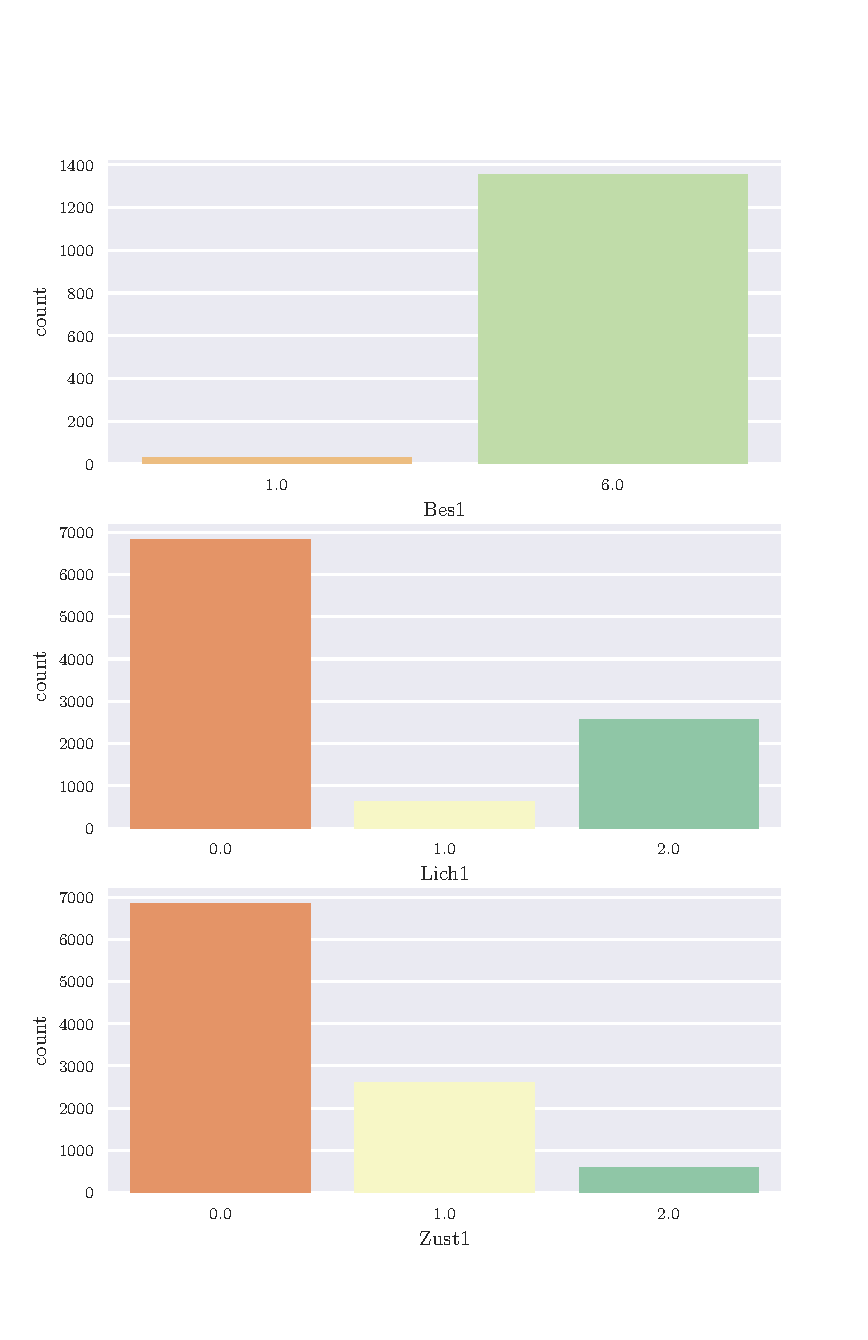
\includegraphics[scale=0.7, trim=0cm 1.5cm 0cm 1cm]{../CorrAnalysis/data/BAYSIS/01_dataset/plots/baysis_dataset_count_multiple04}
	\caption{Distribution of the accident category Zust, Fstf and WoTag}
	\label{img:baysis_dataset_Zust_Fstf_WoTag}
\end{figure}
\pagestyle{headings}
	
\bigskip
	
\begin{table}[ht]
	\centering
	\begin{tabular}{c|c|c|c}
		\textbf{Variable} 	& \textbf{Group} 	& \textbf{Type} & \textbf{Format} \\
		\toprule
		Kat  		& categorical 	& ordinal 	& numeric\\
		\midrule
		Typ 		& categorical 	& nominal	& numeric\\
		\midrule
		Beteil 		& categorical 	& ordinal	& numeric\\
		\midrule
		UArt 		& categorical 	& nominal	& numeric\\
		\midrule
		AUrs 		& categorical 	& nominal	& numeric\\
		\midrule
		AufHi 		& categorical 	& nominal	& numeric\\
		\midrule
		Alkoh 		& categorical 	& dichotomous	& numeric\\
		\midrule
		Char 		& categorical 	& nominal	& numeric\\
		\midrule
		Bes 		& categorical 	& nominal	& numeric\\
		\midrule
		Lich 		& categorical 	& ordinal	& numeric\\
		\midrule
		Zust 		& categorical 	& ordinal	& numeric\\
		\midrule
		Fstf 		& categorical 	& nominal	& mixed\\
		\midrule
		WoTag 		& categorical 	& nominal	& text\\
		\midrule
		FeiTag 		& categorical 	& dichotomous	& numeric\\
		\bottomrule
	\end{tabular}
	\caption{Variable types of \acrshort{baysis} dataset}
	\label{tab:table_baysis_paramters}
\end{table}

Table \autoref{tab:table_baysis_paramters} show all categorized parameters, relevant for the correlation analysis, with variable group, type and the format of the containing data. To check for dependent variables which need to be considered in a correlation analysis, the correlation matrix for all relevant parameters in the BAYSIS dataset is calculated (see figures/tables \autoref{img:correlation_matrix_dataset_cramers}/\autoref{table:appendix_correlation_matrix_dataset_cramers} for Cramer's $V$ and \autoref{img:appendix_correlation_matrix_dataset_theils}/\autoref{table:appendix_correlation_matrix_dataset_theils} for Theil's $U$). Cramer's $V$ reveals several strong relationships, which are 'Typ'-'UArt1'. 'AUrs1'-'Zust1', 'AUrs1'-'Zust2' and some  trivial relations of 'Char1'-'Char2', 'Bes1'-'Bes2', 'Lich1'-'Lich2'. The results of Theil's $U$ confirms the relationships identified by Cramer's $V$ with a moderate effect size and show the association of 'Aufhi'-'UArt' with a strong effect size. 

% TODO check p-value and 

That means that relations found in the later analysis, which contain the parameters 'Typ', 'UArt1, 'AUrs1, 'Zust1' and 'Zust2' might be in result of another depended variable and should be checked for independence.

% ------- BAYSIS Dataset - Matrix --------
\newgeometry{left=1.5cm,right=1cm}
\pagestyle{empty}
\begin{figure}[ht]
	\centering
	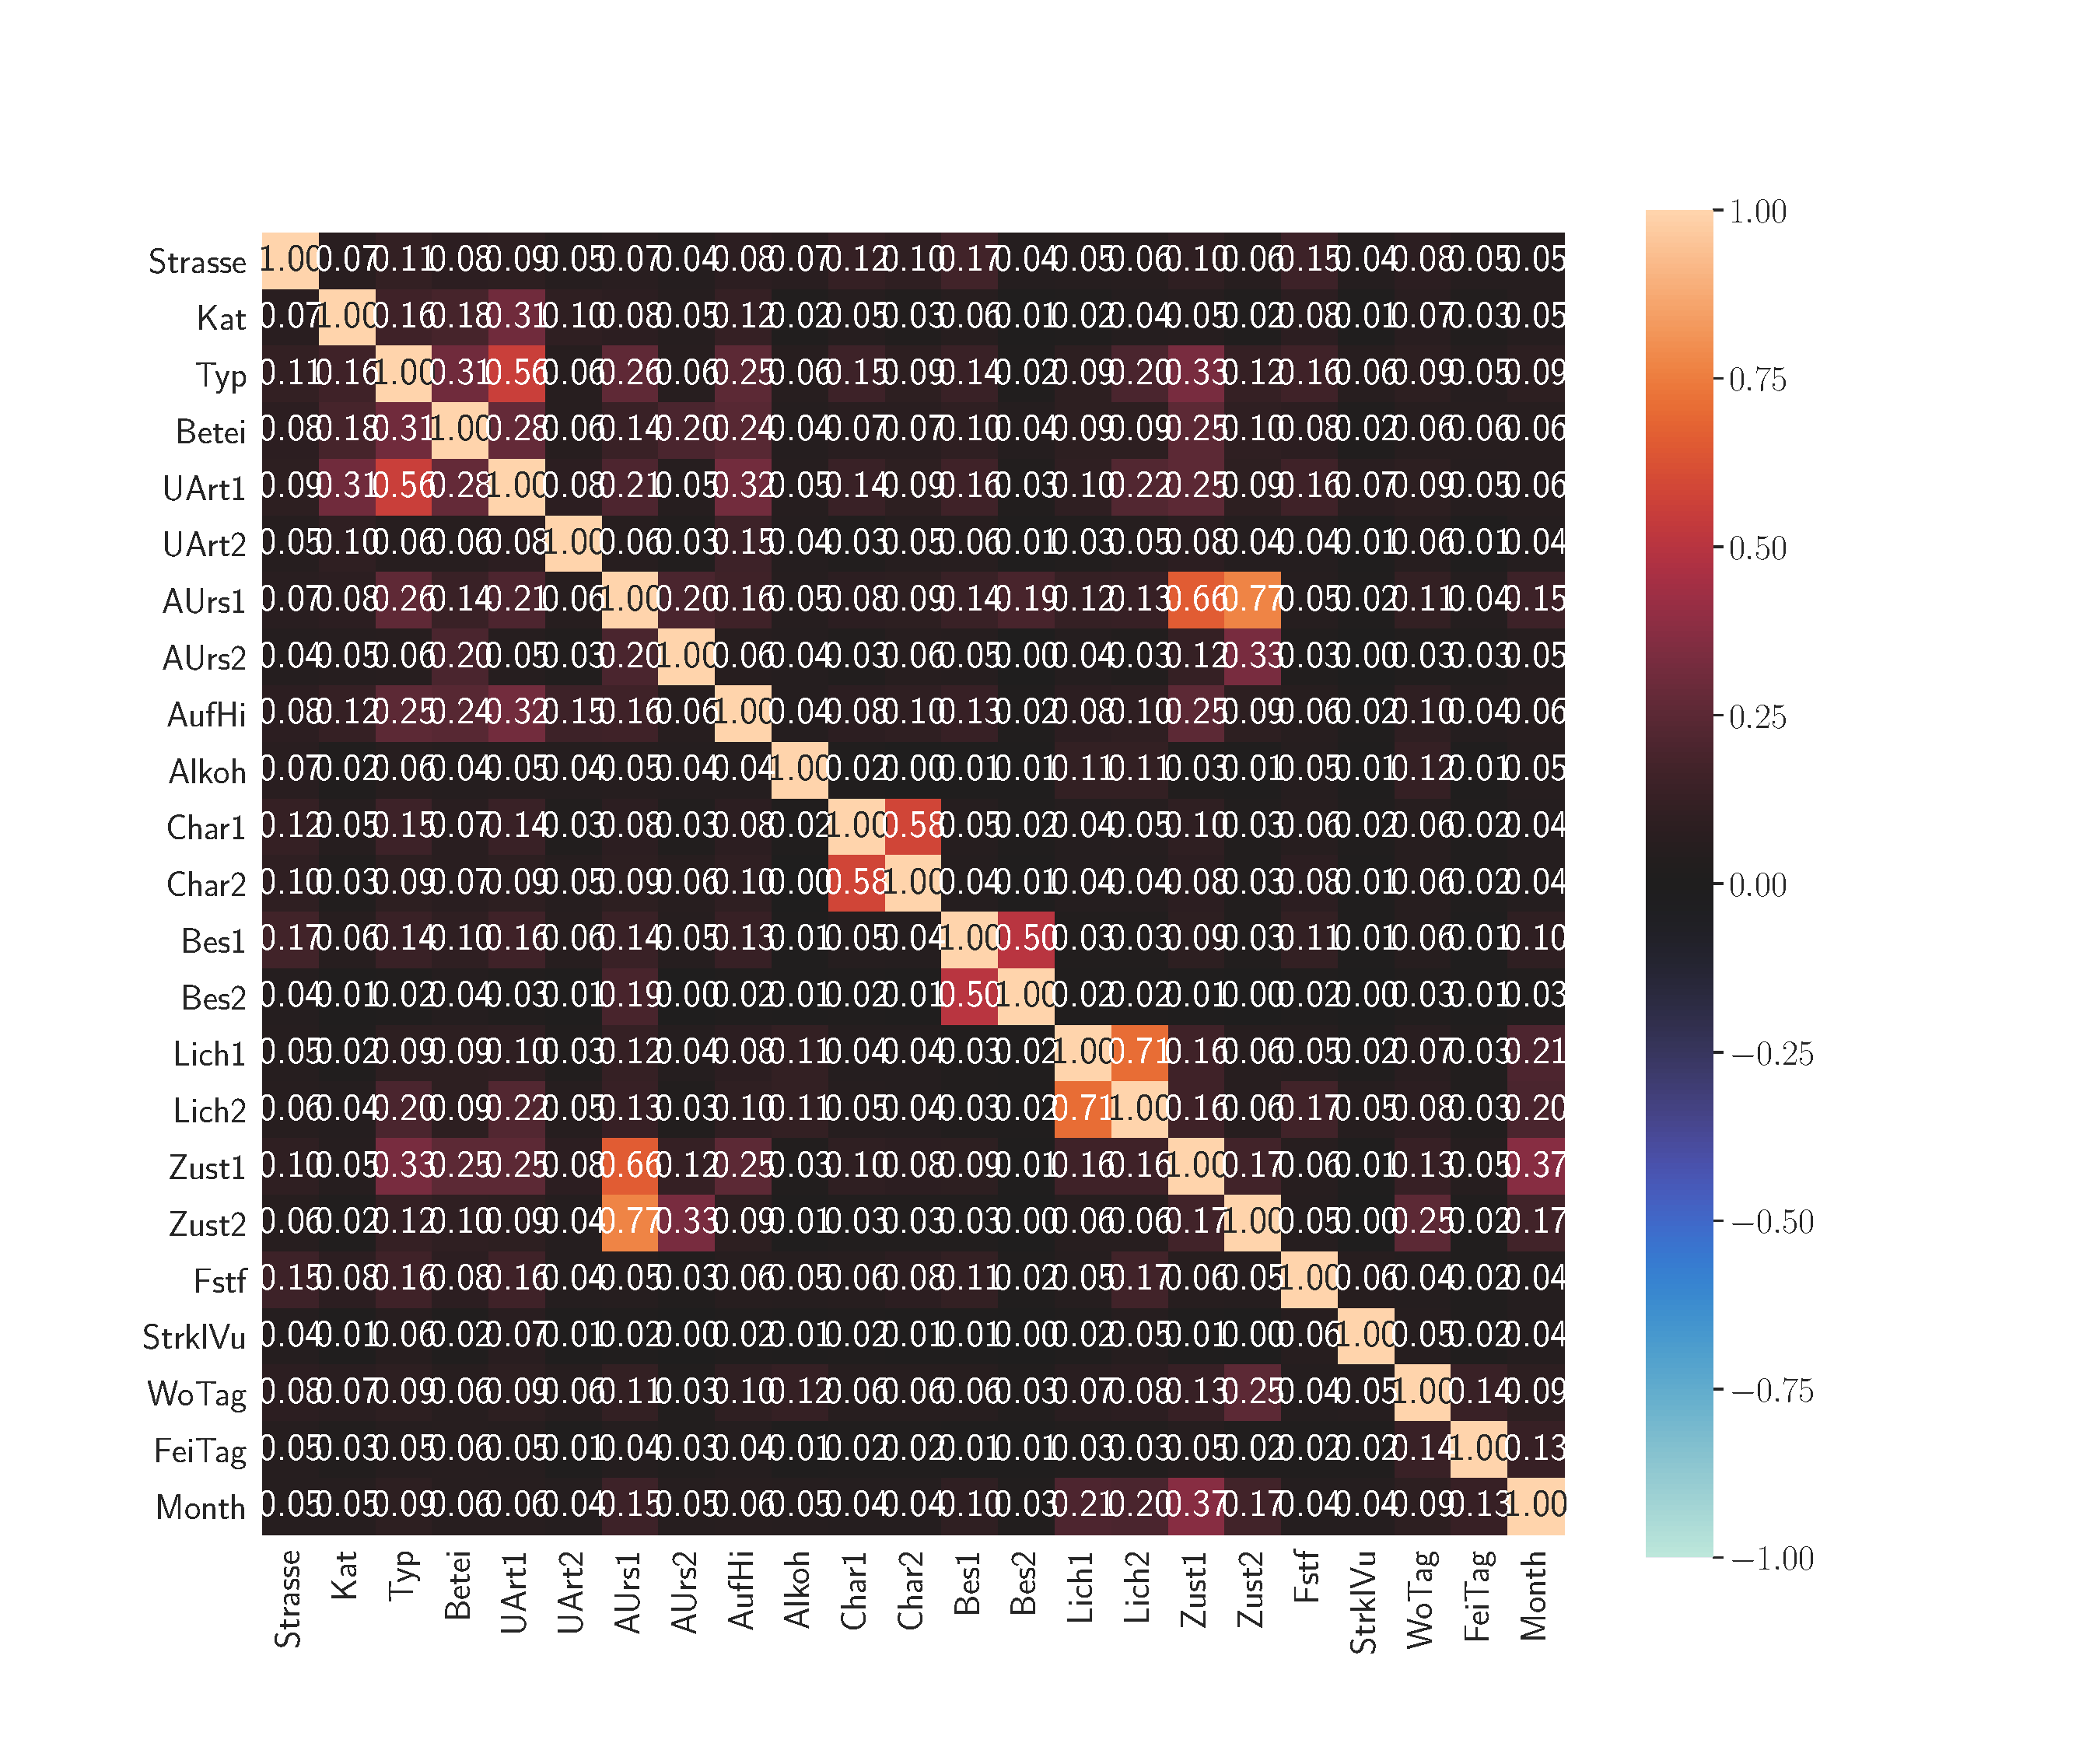
\includegraphics[scale=0.4, trim=4cm 6cm 0cm 6cm]{../CorrAnalysis/data/BAYSIS/01_dataset/plots/baysis_dataset_corr_cramers}
	\caption{Correlation matrix for BAYSIS dataset, with Cramer's $V$}
	\label{img:correlation_matrix_dataset_cramers}
\end{figure}
\restoregeometry
\pagestyle{headings}
%\newgeometry{left=1.5cm,right=1cm}
%\begin{figure}[h]
%	\centering
%	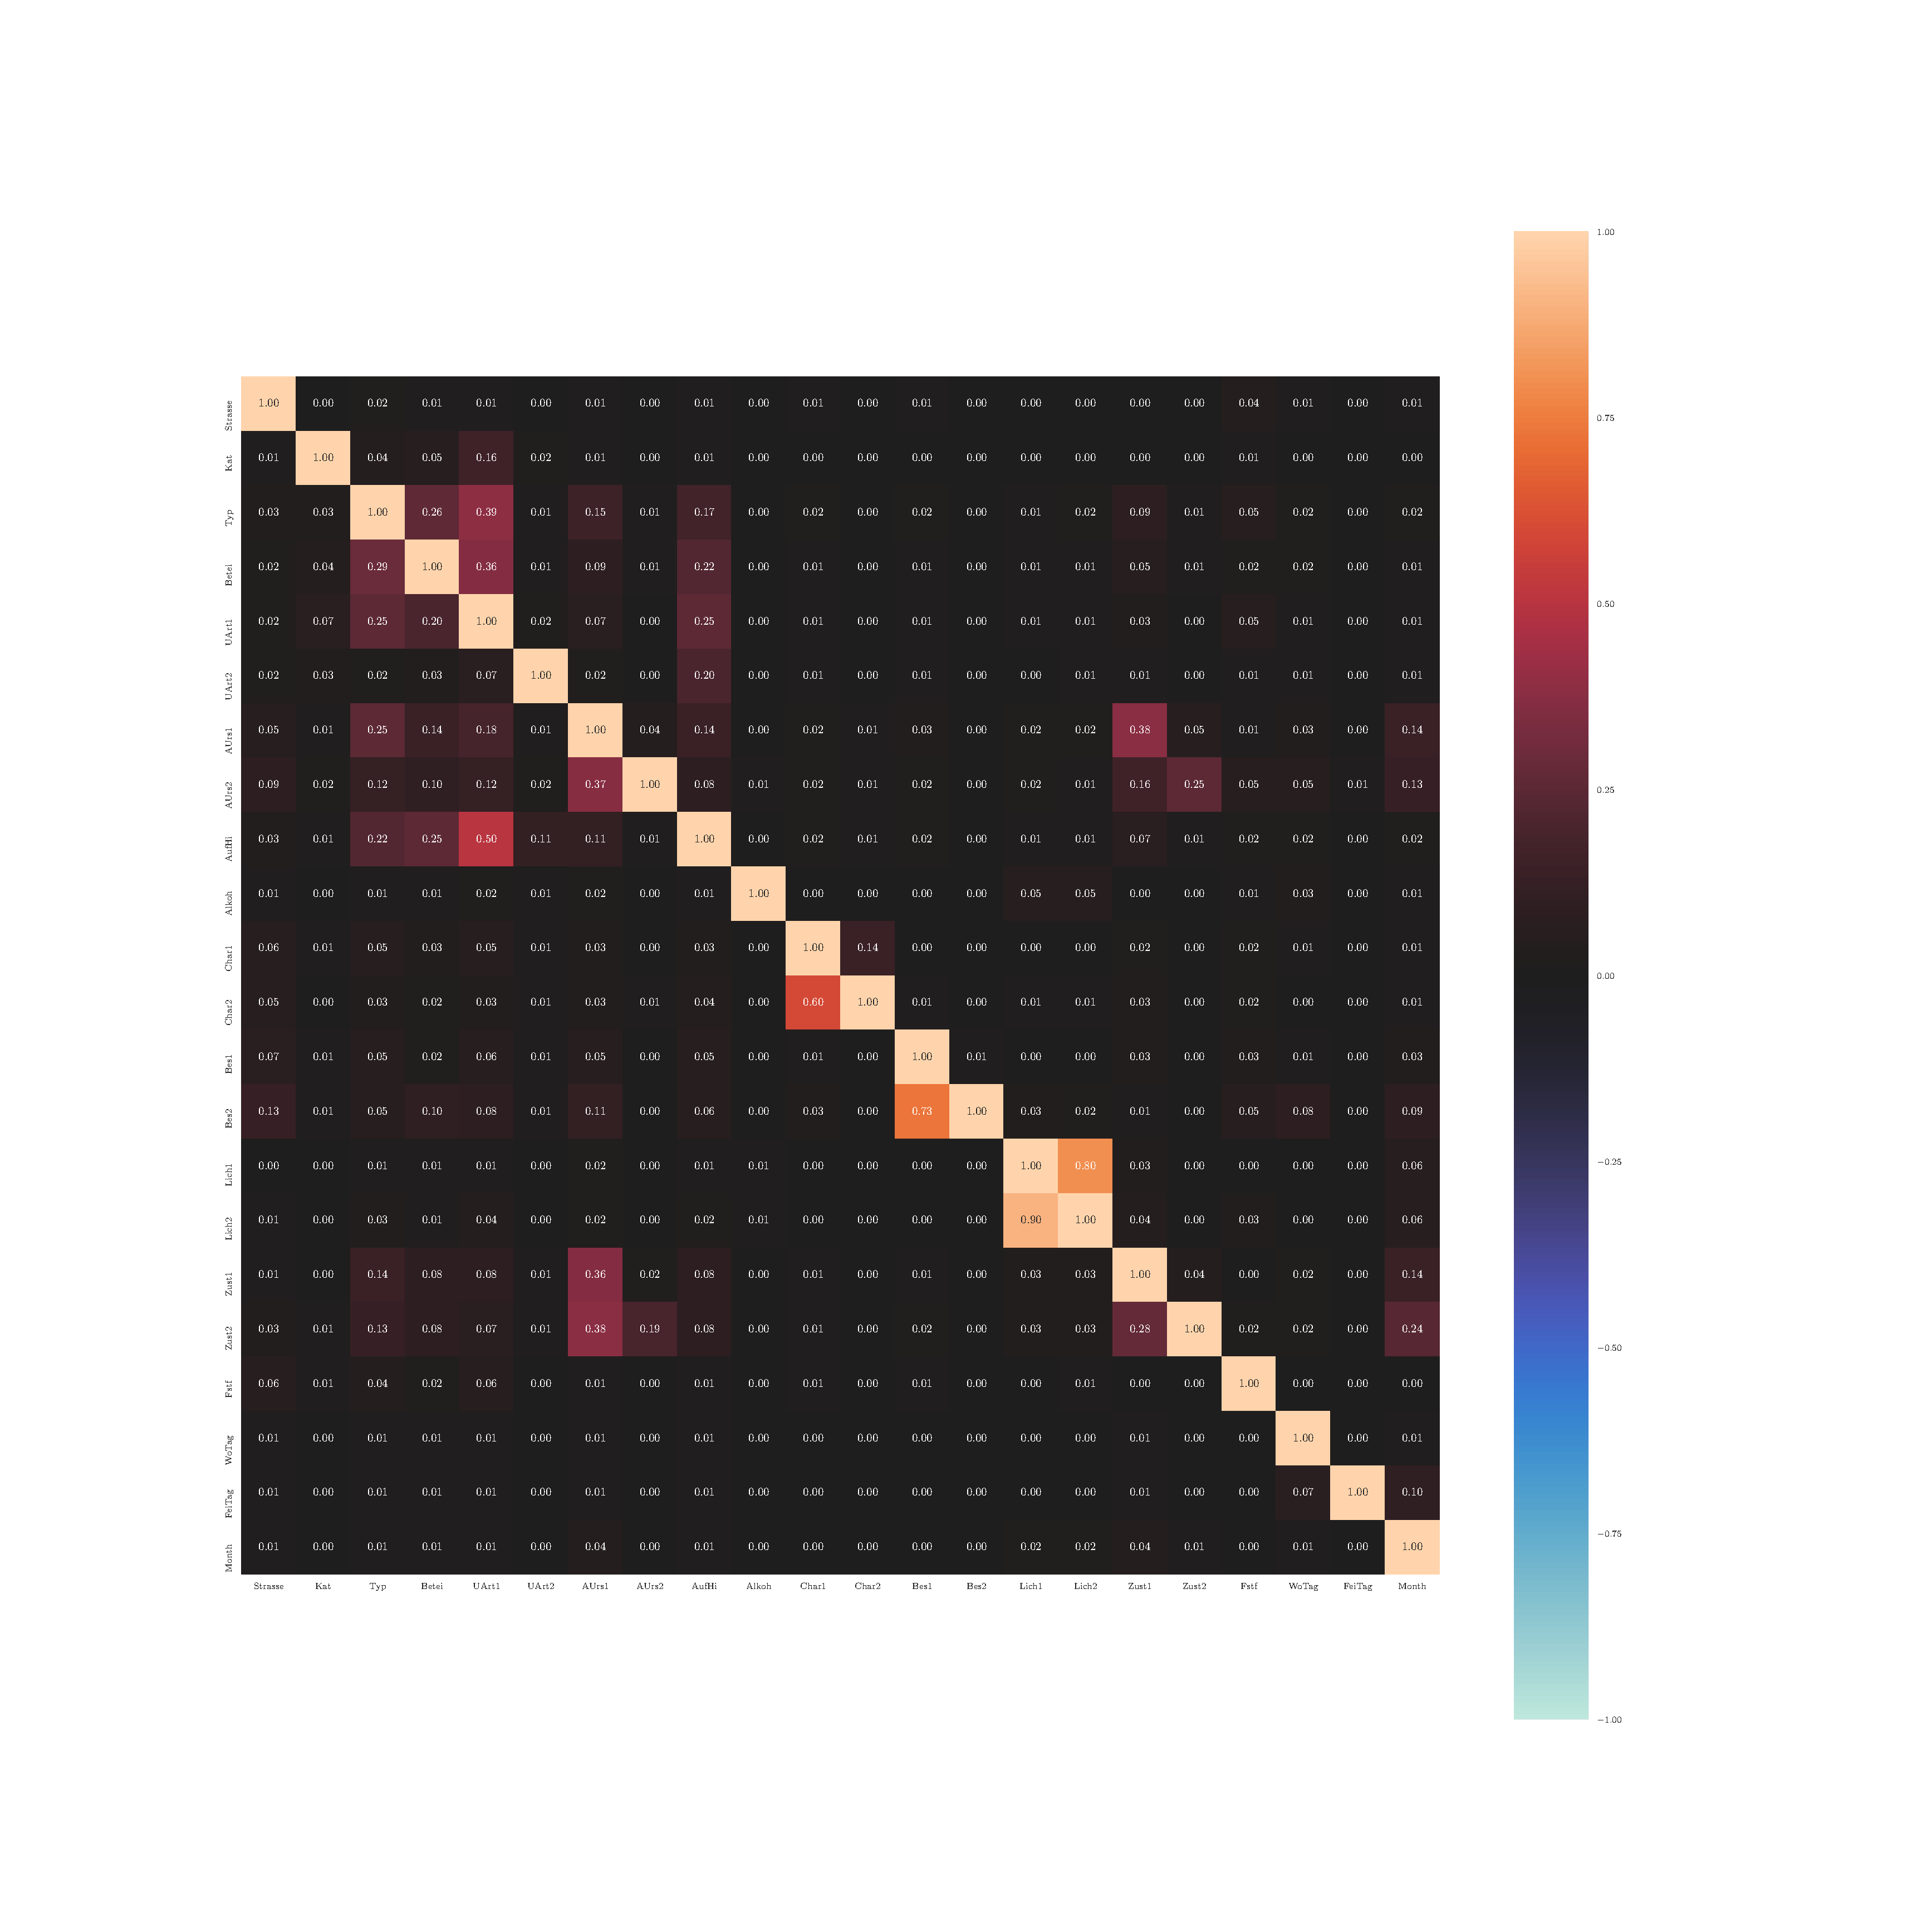
\includegraphics[scale=0.4, trim=2cm 6cm 0cm 6cm]{../CorrAnalysis/data/BAYSIS/01_dataset/plots/baysis_dataset_corr_theils}
%	\caption{Correlation matrix for BAYSIS dataset, with Theil's $U$}
%	\label{img:appendix_correlation_matrix_dataset_theils}
%\end{figure}
%\restoregeometry

The designed evaluation tool, utilizes a PostgreSQL database for its data storage. Therefore the BAYSIS data in form of \acrfull{csv} needs to processed and converted into SQL data entities. Also, the data entities for each accident need to be uniform and comparable with our street network and other entities like roadworks, which makes it necessary to process and map the accidents onto our street network. After the necessary processing and import into the database, 7971 re cords end up being converted and persisted, which equivalent to 77,6\% of the total number of accidents. This 22,4\% of data loss is due to the conversion of from the BAYSIS geo-system to the HERE network, which tries to find a corresponding street network location to the legacy location of the BAYSIS dataset. If it is not able to locate the position of the BYSIS dataset on our street network, the record is discarded.s

\section{ArbIS}
\label{dataset_arbis}

The \acrfull{arbis}, as described in chapter \autoref{dataset_arbis}, is a collection service of all roadworks or maintenance planned, ongoing or finished on the Bavarian street network. With the 4500 long term and more than 40.000 short term building sites on German highways per year \parencite{LAPID2018,Stmi2020}, road construction makes up for the majority of traffic obstructions in the summer months, when during the colder month, in which many kinds of construction projects are not possible, snow clearings or long-term constructions are the issue. That also means that the number and type of roadworks varies during the course of a year \parencite{Stmi2020}.

The dataset for 2019 contains close to 650.000 data-points, which each describe the temporal and spatial extend, road name and number of closed lanes of a roadwork fragment. This fragmentation of events makes is rather hard to statically analyze this dataset since each roadwork is spitted into any number of fragments in now recognizable pattern and are only linked by a roadwork identifier. Therefore the analysis of the dataset in this section is rather basic. The import processing, similarly to the \acrshort{baysis} data in \autoref{dataset_baysis}, and aggregation of fragments produces 282.839 roadwork events in the database. The monthly distribution of roadworks in the year 2019 in figure \autoref{img:arbis_dataset_dist_month} shows that the winter months of January, February and December tend to have less roadwork that others, due to colder temperatures. The month of July has the most roadworks.

\begin{figure}[ht]
	\centering
	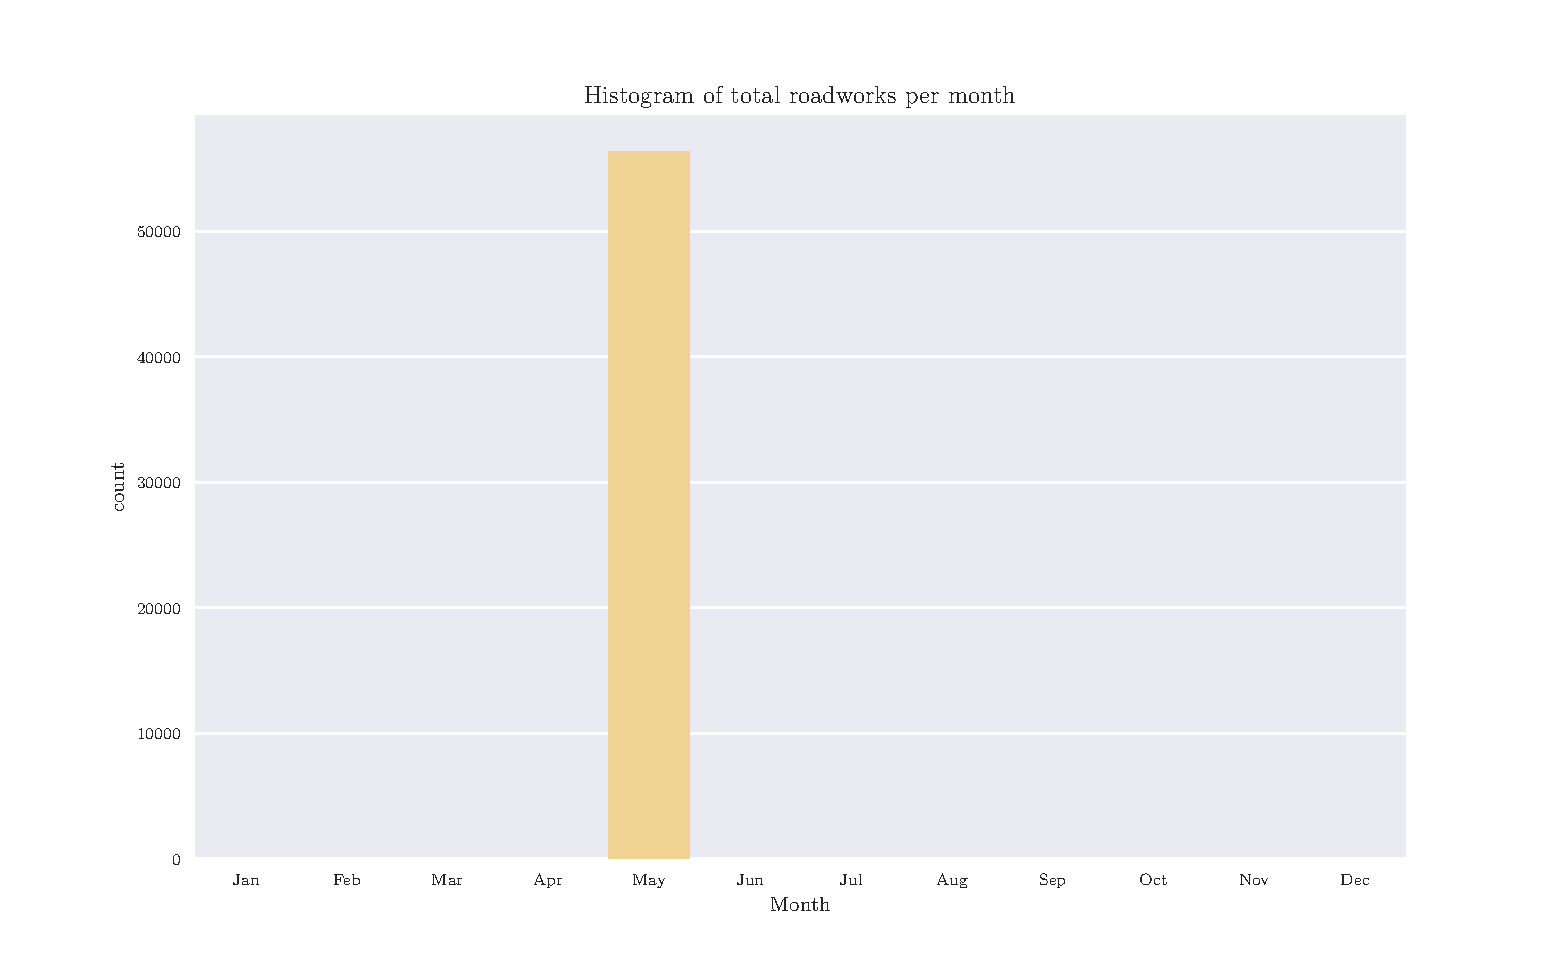
\includegraphics[width=0.7\textwidth]{../CorrAnalysis/data/ArbIS/01_dataset/plots/arbis_dataset_hist_month}
	\caption{Monthly distribution of roadwork fraction counts}
	\label{img:arbis_dataset_dist_month}
\end{figure}

As with the BAYSIS data the counts of roadworks by road (shown in figure \autoref{img:arbis_dataset_dist_highway}) the road "A3" and "A9" have the highest numbers of roadworks.

\begin{figure}[ht]
	\centering
	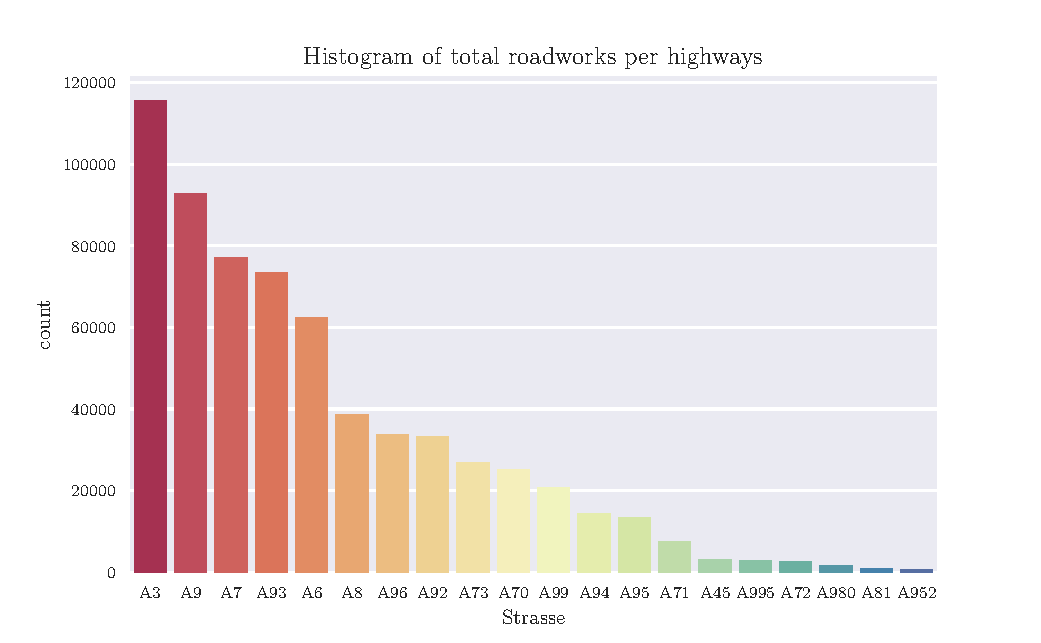
\includegraphics[width=0.7\textwidth]{../CorrAnalysis/data/ArbIS/01_dataset/plots/arbis_dataset_hist_highway}
	\caption{Distribution of roadwork fraction counts, by road}
	\label{img:arbis_dataset_dist_highway}
\end{figure}

\paragraph{AnzGesperrtFs} refers to the number of closed lanes for the time of the incident. The distribution (shown in figure \autoref{}) shows that two categories hold nearly 100\,\%, zero and one block lane. Since there are some samples with two and three closed lane (in total less than .01\,\%) the variable is of ordinal type and not dichotomous.

\paragraph{Einzug} describes the shift of the road way due to physical changes, measured in number of lanes (distribution show in \autoref{}). It ranges from one to five lanes, where one, two and five are equally frequent. 

\paragraph{Length} is calculated from the two dataset parameters 'VonKilometer' and 'BisKilometer'. Is is not part of the original ArbIS dataset.

\paragraph{Duration} is calculated from the two dataset parameters 'Von' and 'Bis'. Is is not part of the original ArbIS dataset.

\bigskip

Table \autoref{table:table_arbis_paramters} show all categorized parameters, relevant for the correlation analysis, with variable group, type and the format of the containing data.
	
\begin{table}[ht]
	\centering
    \begin{tabular}{c|c|c|c}
		\textbf{Variable} 	& \textbf{Group} 	& \textbf{Type} 		& \textbf{Format} \\
		\\[-1em]
		\hline
		\\[-1em]
		AnzGesperrtFs  	& categorical 	& ordinal 	& numeric\\
		\hline
		\\[-1em]
		Einzug  		& categorical 	& ordinal 	& numeric\\
		\hline
		\\[-1em]
		Length  		& continuous 	& interval 	& numeric\\
		\hline
		\\[-1em]
		Duration  		& continuous 	& interval 	& numeric\\
	\end{tabular}
	\caption{Variable types of \acrshort{baysis} dataset}
	\label{table:table_arbis_paramters}
\end{table}
